\documentclass[tikz,border=2pt]{standalone}
\usepackage{amsmath,amssymb}
\usepackage{tikz}
\usetikzlibrary{matrix}

\begin{document}
% Initial simplex tableau of the Giapetto LP in augmented form: objective row written as
% z - 3 x_s - 2 x_t = 0, one row per constraint with its slack as basic variable.
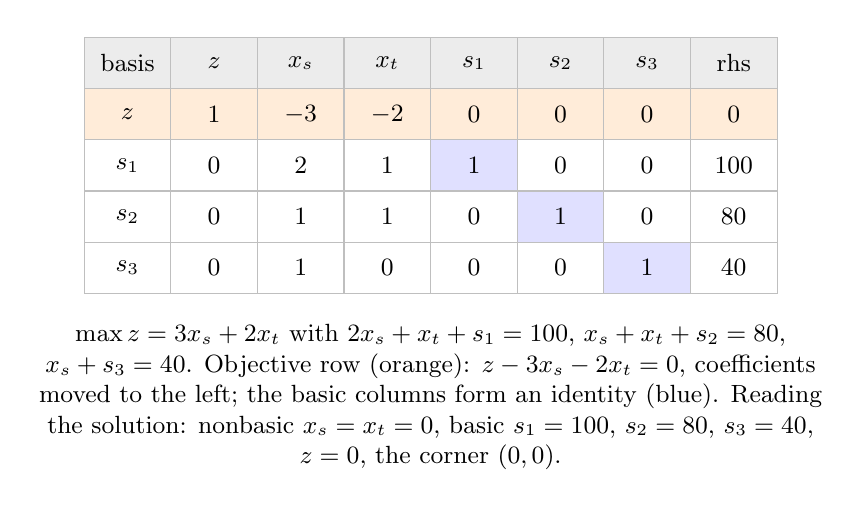
\begin{tikzpicture}[every node/.style={font=\small}]
	\matrix (T) [matrix of math nodes, nodes={minimum width=1.1cm, minimum height=6.5mm, anchor=center, draw=gray!50}, column sep=-\pgflinewidth, row sep=-\pgflinewidth] at (0,0) {
		|[fill=gray!15]| \text{basis} & |[fill=gray!15]| z & |[fill=gray!15]| x_s & |[fill=gray!15]| x_t & |[fill=gray!15]| s_1 & |[fill=gray!15]| s_2 & |[fill=gray!15]| s_3 & |[fill=gray!15]| \text{rhs} \\
		|[fill=orange!15]| z & |[fill=orange!15]| 1 & |[fill=orange!15]| -3 & |[fill=orange!15]| -2 & |[fill=orange!15]| 0 & |[fill=orange!15]| 0 & |[fill=orange!15]| 0 & |[fill=orange!15]| 0 \\
		s_1 & 0 & 2 & 1 & |[fill=blue!12]| 1 & 0 & 0 & 100 \\
		s_2 & 0 & 1 & 1 & 0 & |[fill=blue!12]| 1 & 0 & 80 \\
		s_3 & 0 & 1 & 0 & 0 & 0 & |[fill=blue!12]| 1 & 40 \\
	};
	\node[anchor=north, align=flush center, text width=10cm] at ([yshift=-4pt]T.south) {$\max z=3x_s+2x_t$ with $2x_s+x_t+s_1=100$, $x_s+x_t+s_2=80$, $x_s+s_3=40$. Objective row (orange): $z-3x_s-2x_t=0$, coefficients moved to the left; the basic columns form an identity (blue). Reading the solution: nonbasic $x_s=x_t=0$, basic $s_1=100$, $s_2=80$, $s_3=40$, $z=0$, the corner $(0,0)$.};
\end{tikzpicture}
\end{document}
